\section{Evaluation der Implementation mit echten Logdateien}
In diesem Abschnitt verwendeten wir unsere Implementierung für die Analyse von \gls{ssh}-Logdateien der Hochschule. Für die Extrahierung der Dateien bekommt unseren Promtail-Instanz folgende Konfiguration:

{\setstretch{1.0}
\begin{Verbatim}[frame=single,fontsize=\small]
scrape_configs:
- job_name: sshlogs
  decompression:
    enabled: true
    initial_sleep: 15s
    format: gz
  static_configs:
  - targets:
      - localhost
    labels:
      job: sshlogs
      instance: Opfersystem1
      __path__: /var/log/**.gz
\end{Verbatim}
}

Promtail sucht automatisch und nach vordefinierten Zeitabstand nach Logdateien, die in der Konfigurationsdatei eintregagen wurden. In der Tabelle \ref{tab:KonfigPromtail} befindet sich die Erklärung jedes Elements dieser Konfiguration:

\begin{table}[H]
    \setstretch{1}
    \begin{tabularx}{\textwidth}{|m{5.5cm}|X|}
    \hline
    \multicolumn{1}{|c|}{\textbf{Konfigurationsfeld}} & \multicolumn{1}{|c|}{\textbf{Beschreibung}} \\
    \hline
    scrape\_configs & Bezieht sich auf die Funktionalität von Promtail automatisch nach Logdatein zu suchen. \\
    \hline
    decompression \newline
    \hphantom{12}enabled: true \newline
    \hphantom{12}initial\_sleep: 10s \newline
    \hphantom{12}format: gz & Promtail kann die einige Komprimierungsformate verarbeiten, unter denen .gz, was wir in unserer Arbeit benutzen. Der field \quotes{initial\_sleep} beschreibt die Intervallzeit, bevor die Dekomprimierung anfängt. Dieser Felt kann nützlich sein, wenn komprimierte Datei vorhanden sind aber deren Komprimierungsverfahren noch nicht abschlossen ist. Der Feld Format deutet auf die Komprimierungsformate hin \citep{Grafana_Promtail}.  \\
    \hline
    \end{tabularx}
\end{table}

\begin{table}[H]
  \setstretch{1}
  \begin{tabularx}{\textwidth}{|m{5.5cm}|X|}
  \hline
  \multicolumn{1}{|c|}{\textbf{Konfigurationsfeld}} & \multicolumn{1}{|c|}{\textbf{Beschreibung}} \\
  \hline
  static\_configs: \newline
  \hphantom{1}- targets: \newline
  \hphantom{123}- localhost \newline
  \hphantom{1}labels: \newline
  \hphantom{123}job: sshlogs \newline
  \hphantom{123}\_\_path\_\_: /var/log/**.gz & \quotes{targets} bezieht sich auf die Kommunikation mit dem Loki-Instanz. \quotes{labels} zeigt, mit welcher Identifizierung den Inhalt dieser Datei im Loki aufgerufen werden kann. \quotes{\_\_path\_\_} gibt an, wo sich die Datei im System befinden\\
  \hline
  %sample\_rate: 0.1 & , which means that Promtail will sample 10% of the series during scraping. \\
  %\hline
  \end{tabularx}
  \caption[Konfigurationsausschnitt von Promtail]
  {Konfigurationsausschnitt von Promtail}
  \label{tab:KonfigPromtail}
\end{table}

\quotes{Labels} spielen eine wesentliche Rolle in der Performance bei Loki, da dieses Tool mit weniger Indexierung als anderes Tool, wie Elastic Stack, arbeitet. \cite{Grafana_labels} empfiehl so wenig \quotes{labels} wie möglich zu verwenden, die Extrahierung von Inhalt sollte stattdessen mithilfe der \gls{abfragesprache} stattfinden, um eine Eskalation bei der Speicherung zu vermeiden. Die Abbildung \ref{fig:Eskalation_Labels} zeigt den Effekt von mehreren Labels auf die Anwendung:

\begin{figure}[H]
  \centering
  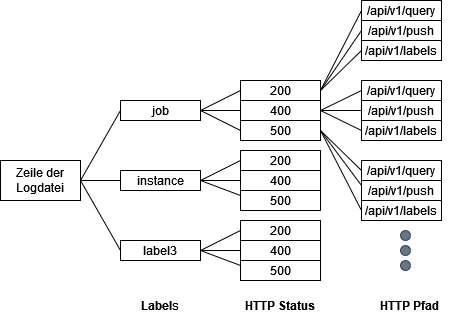
\includegraphics[width=0.7\textwidth]{assets/labelstream.png}
  \caption[Eskalation bei der Indexierung]
  {Eskalation bei der Indexierung Labels laut \cite{Grafana_labels}}
  \label{fig:Eskalation_Labels}
  \centering
\end{figure}

Auf der Abbildung \ref{fig:Eskalation_Labels} haben wir vier Ebenen. Die erste ist die Zeile der Logdatei (1), die zweite ist die von den Benutzer definierten \quotes{labels} (2) und die dritte und vierte beziehen sich auf die Antwort (3) und auf die verwendeten \gls{http}-Anfrage (4), um nach Inhalt abzufragen, hinzuzufügen und zu indexieren. Aus einer Zeile der Logdatei definierten wir drei \quotes{labels} (3x), diese haben wiederum drei potentielen Status (3x3x) aus drei notwendigen \gls{http}-Pfad (3x3x3). Aus einer Zeilen hätten wir schließlich 27 Streams, um die Zeile zu lesen, zu indexieren und zu speichern. Das kann laut \cite{Grafana_labels} zu mangelnden Leistungsfähigkeit führen.

Unsere Logdateien haben ungefähr vier Megabyte, was eine kleine Menge entspricht, wenn man an produktive Umgebung denkt, wo Logdateien schon den Terabyte-Bereich erreichen. Trotz dieser Größe, war unsere Synchronisation nicht immer präziser als erwartet. Einige Abfrage, die bei der Implementierung mit 40 KB Logdateien einwandfrei funktionierten, lieferten hier folgende Fehlermeldung:

{\setstretch{1.0}
\begin{Verbatim}[fontsize=\small, frame=single]
maximum of series (500) reached for a single query  
\end{Verbatim}
}

Die offiziele Dokumentation und die verschiedenen Forums waren nicht in der Lage, uns eine endgültige Lösung mit den neusten Version von Loki (2.8.2) anzubieten. Die verschiedenen Konbination in der Konfigurationsdatei von Loki lieferten immer dasselbe Ergebnis. Bei der Zeit, in der wir uns mit diesem Teil der Arbeit beschäftigen (19.5.2022), versuchten wir, im Kontakt mit dem Team von Grafana Loki über den Forum von Github zu setzen, um eine mögliche Fehlerbehebung zu finden.

Mit der Nutzung von Versiom (2.4.1) konnten wir die obigen Situation teilweise lösen. Unsere Abfrage wurde erfolgreich geschickt und die Graphiken wurden auch generiert. Die folgende Konfigurations-Schnipsel von Loki trug dazu bei, die Leistungsparameter der Anwendungen zu definieren:

{\setstretch{1.0}
\begin{Verbatim}[fontsize=\small, commandchars=\\\{\},frame=single]
\textbf{\textcolor{blue}{limits_config:}}
  reject_old_samples: true
  reject_old_samples_max_age: 168h
  ingestion_rate_mb: 1024
  ingestion_burst_size_mb: 1024
  ingestion_rate_strategy: local
  per_stream_rate_limit: 12MB
  max_query_series: 100000
  max_query_parallelism: 32
  split_queries_by_interval: 24h
  max_query_length: 0h

\textbf{\textcolor{blue}{querier:}}
  max_concurrent: 2048

\textbf{\textcolor{blue}{frontend:}}
  max_outstanding_per_tenant: 4096
  compress_responses: true
  scheduler_worker_concurrency: 20


\textbf{\textcolor{blue}{chunk_store_config:}}
  max_look_back_period: 0s

\textbf{\textcolor{blue}{table_manager:}}
  retention_deletes_enabled: false
  retention_period: 360s
\end{Verbatim}
}

Die Bedeutung unsere Einstellung befindet sich in der Tabelle \ref{tab:KonfigLoki}:
\begin{table}[H]
  \setstretch{1}
  \begin{tabularx}{\textwidth}{|p{7cm}|X|}
  \hline
  \multicolumn{1}{|c|}{\textbf{Konfigurationsfeld}} & \multicolumn{1}{|c|}{\textbf{Beschreibung}} \\ \hline
  \textbf{limits\_config:} & Festlegung der Aufnahmerate; \\
  \hphantom{10}reject\_old\_samples: true & Aufnahme von alten Proben;\\ 
  \hphantom{10}reject\_old\_samples\_max\_age: 168h & Alte Proben werden aufgenommen, wenn diese Alte haben;\\
  \hphantom{10}ingestion\_rate\_mb: 1024 & Aufnahmerate pro Sekunde;\\ 
  \hphantom{10}ingestion\_burst\_size\_mb: 1024 & Aufnahmerate bei einer einzigen Weiterleitung; \\ 
  \hphantom{10}ingestion\_rate\_strategy: local & Aufnahmerate wird \quotes{local} definiert oder \quotes{global} aufgeteilt;  \\ 
  \hphantom{10}per\_stream\_rate\_limit: 12MB & Aufnahmerate in Byte pro Sekunde und pro Strom; \\ 
  \hphantom{10}max\_query\_series: 100000 & Maximal einzelne Serie by Abfrage nach Messwerte; \\ 
  \hphantom{10}max\_query\_parallelism: 32 & Maximale Anzahl von parallelen Abfrage; \\ 
  \hphantom{10}split\_queries\_by\_interval: 24h & Trennung von Abfrage nach einem definierten Intervall;\\ 
  \hphantom{10}max\_query\_length: 0h & Grenze für die Ausführungszeit. Das vermeidet eine Auslastung der Rechenkapazität; \\ 
  \bottomrule
  \end{tabularx}
\end{table}

\begin{table}[H]
  \setstretch{1}
  \begin{tabularx}{\textwidth}{|b{7cm}|X|}
  \hline
  \multicolumn{1}{|c|}{\textbf{Konfigurationsfeld}} & \multicolumn{1}{|c|}{\textbf{Beschreibung}} \\ \hline
  \textbf{querier:} & Einstellung für die Abfrage; \\ 
  \hphantom{10}max\_concurrent: 2048 & Anzahl von konkurrierenden Abfragen;\\ \hline
  \textbf{frontend:} & Einstellung für die Abfrage im \gls{frontend};\\
  \hphantom{10}compress\_responses: true & Komprimierung der \gls{http}-Antworten;\\
  \hphantom{10}scheduler\_worker\_concurrency: 20 & Anzahl von gleichzeitigen Abfragen, die verarbeitet werden; \\  \hline
  \textbf{table\_manager:} & Verwaltung der Vorratsdatenspeicherung;\\ 
  \hphantom{10}retention\_deletes\_enabled: false & Löschung von Tabellen der Datenbank;\\ 
  \hphantom{10}retention\_period 360s & Die Tabellen werden gelöscht, wenn sie älter als dieser Wert sind;\\ \hline
  \bottomrule
  \end{tabularx}
  \caption[Konfigurationsausschnitt für Loki]
  {Konfigurationsausschnitt für Loki}
  \label{tab:KonfigLoki}
\end{table}

Trotz dieser Situation, waren wir in der Lage eine Allgemeine Warnmeldung für hohe Anzahl von fehlgeschlagenen Anmeldeversuche.




% \newpage
% \newgeometry{right=30mm, left=30mm} 
% \thispagestyle{lscape}
% \begin{landscape}
%    Nach manuellen Aktualiserung sah unsere Graphik so aus:
%     \begin{figure}[H]
%        % \centering
%         \centerline{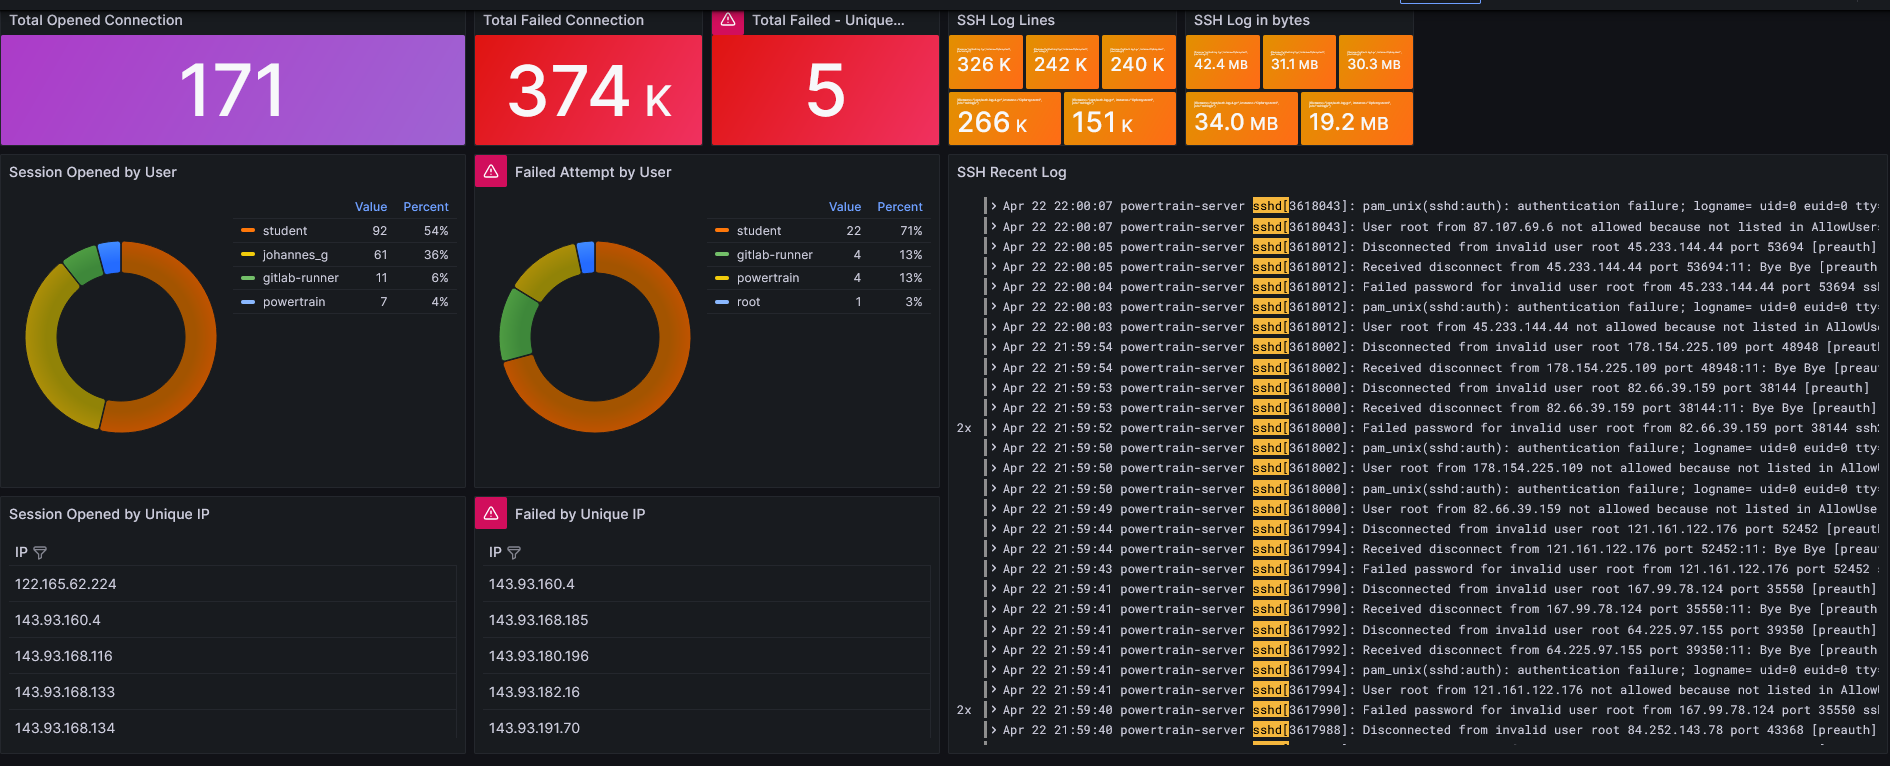
\includegraphics[width=1.8\textwidth]{assets/unserssh}}
%         %\includegraphics[width=1.2\textwidth]{assets/5.4.2_1_Abb.jpeg}
%         \caption[Ausgabe in Grafana von unseren \gls{ssh} Logdateien]
%         {Ausgabe in Grafana von unseren \gls{ssh} Logdateien}
%         \label{fig:Unserssh}
%         \centering
%     \end{figure} 
% \end{landscape}
% \restoregeometry


